%----------------------------------------------------------------------------------------

\begin{frame}
\frametitle{
\includegraphics[scale=0.4]{./materials/Genma.jpg} \ \ \  About me }
\begin{columns}[c] 

\column{.55\textwidth} 
\textbf{Where can you find me on Internet?}
\begin{itemize}
\item Blog (in French) : http://genma.free.fr
\item Twitter : http://twitter.com/genma
\end{itemize}

\textbf{My Hobbies? Many things}
\begin{itemize}
\item Crypto
\item Privacy
\end{itemize}

\column{.5\textwidth} 
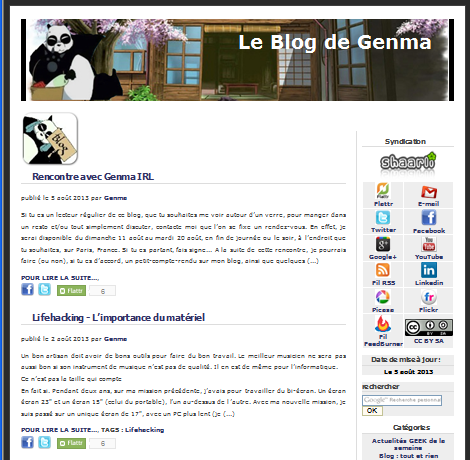
\includegraphics[width=5cm,height=5cm]{./materials/blog.png} 
\end{columns}
\end{frame}


%----------------------------------------------------------------------------------------
\begin{frame}
\frametitle{Digital identity, what is it?}

\begin{block}{Definition}
\begin{itemize}
\justifying{
\item Digital identity is all the public data you can find about someone using Internet research.
\item It's the famous e-reputation.
}
\end{itemize}
\end{block}
\begin{center}

\includegraphics[scale=0.5] {./materials/On-The-Internet-Nobody-Knows-Youre-A-Dog.jpg}
\end{center}

\end{frame}

%----------------------------------------------------------------------------------------
\begin{frame}
\frametitle{What do you think of me?}

\justifying{
\begin{block}{Google you name}
\begin{itemize}
\item The results shown are they exactly what you want?
\end{itemize}
\end{block}
}
\begin{center}
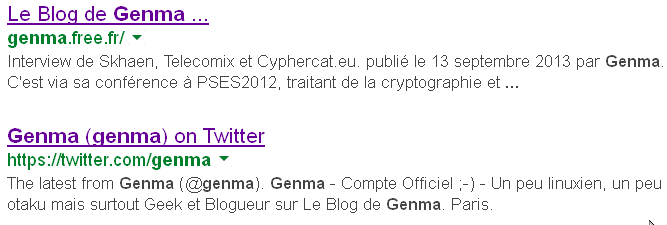
\includegraphics[scale=0.3] {./materials/Google01.png}
\\
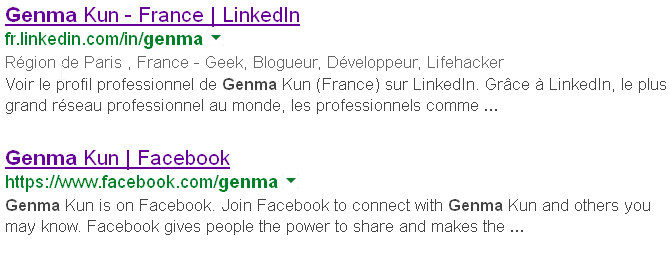
\includegraphics[scale=0.3] {./materials/Google02.png}
\end{center}
\end{frame}

%----------------------------------------------------------------------------------------
\begin{frame}
\frametitle{Saying}

\begin{block}{Words fly, writings remain}
\begin{itemize}
\justifying{
\item This adage is especially true with the Internet.
\item It must be assumed that what is said will always be accessible, even years later.
\item Everything on the Internet is public or will be (even if it is "private", Terms of Use may change).
\item it is therefore not an abuse of freedom of expression and it remains respectful
    of laws
}
\end{itemize}
\end{block}


\end{frame}

%----------------------------------------------------------------------------------------
\begin{frame}
\frametitle{Pseudonymity}


\begin{block}{Defintion}
\begin{itemize}
\justifying{
\item Contraction of anonymity and pseudonym words, the term pseudonymity reflects quite well the contradictory of \textbf{being a public figure and to remain anonymous} ...
\item Have a pseudonym does not mean to say and do anything.
\item This is the image that I return, this is my credibility (past, present and future).
\item A pseudonym is also a public identity, which is associated with different account: my blog, my Twitter, my Facebook account.
\item The digital identity are all these public data associated with this identity.
}
\end{itemize}
\end{block}

\end{frame}


%----------------------------------------------------------------------------------------
\begin{frame}
\frametitle{Samples}

\begin{block}{Twitter}
\begin{center}

\includegraphics[scale=0.2] {./materials/Twitter.png}
\end{center}
\end{block}

\begin{block}{Linkedin}
\begin{center}
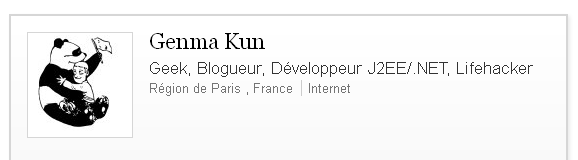
\includegraphics[scale=0.3] {./materials/Linkedin.png}
\end{center}
\end{block}
\end{frame}


%----------------------------------------------------------------------------------------
\begin{frame}
\frametitle{Pseudonymity is disapearing...}

\justifying{
\begin{block}{Facebook}
\begin{itemize}
\item Facebook doesn't allow the creation of an account with a pseudonym,
    if you really want there is some easy steps to follow.
\item The goal is to force people to express themselves using their real names,
\end{itemize}
\end{block}
}

\end{frame}

%----------------------------------------------------------------------------------------
\begin{frame}
\frametitle{Pseudonymity is seen as a problem}

\justifying{
The problem is that the anonymity is taken as an excuse to condemn the use of the Internet as a tool for freedom of expression. 
\\
If people are monitored, they do not say what they think, they do not criticize the politicians. 
\\
With the Internet, the citizen is gradually taking power on politicians.
}

\end{frame}

%----------------------------------------------------------------------------------------
\begin{frame}
\frametitle{Conclusion}
\justifying{
\begin{block}{Pseudonymity is a necessity}
\begin{itemize}
\item Manage your digital identity.
\item \textbf{Pseudonymity is the first step to take back you privacy.}
\end{itemize}
\end{block}
}

\end{frame}

